%%%%%%%%%%%%%%%%%%%%%%%%%%%%%%%%%%%%%%%%%%%%%%%%%%%%%%%%%%%%%%%%%%%%
%%%           Vorlage für eine Ausarbeitung an der DHBW          %%%
%%%                                                              %%%
%%%      Bereiche die bearbeitet werden müssen werden durch      %%%
%%%      einen solchen Kommentarblock eingeleitet und enden      %%%
%%%      mit der nächsten Trennlinie.                            %%%
%%%                                                              %%%
%%%      In dieser Datei müssen folgende Bereiche bearbeitet     %%%
%%%      werden:                                                 %%%
%%%      - Angaben zur Arbeit                                    %%%
%%%      - EIGENE KAPITEL EINFÜGEN                               %%%
%%%                                                              %%%
%%%      Benötigte Seiten und Verzeichnisse können unter         %%%
%%%      "Einführung und Verzeichnisse" ein- bzw. auskommentiert %%%
%%%      werden.                                                 %%%
%%%                                                              %%%
%%%%%%%%%%%%%%%%%%%%%%%%%%%%%%%%%%%%%%%%%%%%%%%%%%%%%%%%%%%%%%%%%%%%

\documentclass[a4paper,12pt]{article}
\usepackage[left=2.5cm,right=2.5cm,top=2.5cm,bottom=2.5cm,includehead]{geometry}      % Einstellungen der Seitenränder
\usepackage[english, ngerman]{babel}                                                  % deutsche Silbentrennung
\usepackage[utf8]{inputenc}                                                           % Umlaute
\usepackage[official]{eurosym}                                                        % Euro Symbol
\usepackage[T1]{fontenc}													                                    % Umlaute auch richtig ausgeben
\usepackage{newtxtext,newtxmath}                                                      % Font = Times New Roman
\usepackage{hyperref}
\usepackage[nottoc]{tocbibind}
\usepackage{fancyhdr}
\usepackage{setspace}
\usepackage[backend=bibtex, citestyle=authoryear, bibstyle=authoryear]{biblatex}      % Bibliothek für Zitate
\usepackage{csquotes}                                                                 % Zusatzpacket für Zitate
\usepackage{amsmath}                                                                  % Zurücksetzen der Tabellen- und Abbildungsnummerierung je Sektion
\usepackage[labelfont=bf,aboveskip=1mm]{caption}                                      % Bild- und Tabellenunterschrift (fett)
\usepackage[bottom,multiple,hang,marginal]{footmisc}                                  % Fußnoten [Ausrichtung unten, Trennung durch Seperator bei mehreren Fußnoten]
\usepackage{graphicx}  
\graphicspath{{./images/}}                                                            % Grafiken
\usepackage[dvipsnames]{xcolor}                                                       % Farbige Buchstaben
\usepackage{wrapfig}                                                                  % Bilder in Text integrieren
\usepackage{enumitem}                                                                 % Befehl setlist (Zeilenabstand für itemize Umgebung auf 1 setzen)
\usepackage{listings}                                                                 % Quelltexte
\definecolor{commentgreen}{RGB}{87,166,74}                                            % Kommentar-Farbe für Quellcode
\lstset{numbers=left, numberstyle=\tiny, numbersep=8pt, frame=single, framexleftmargin=15pt, breaklines=true, commentstyle=\color{commentgreen}}
\usepackage{tabularx}                                                                 % Tabellen
\usepackage{multirow}                                                                 % Mehrzeilige Tabelleneinträge
\usepackage[addtotoc]{abstract}                                                       % Abstract
\usepackage[nohyperlinks, printonlyused, withpage]{acronym}                           % Abkürzungen
\usepackage{dirtree}                                                                  % Ordnerstruktur (z.B. für Anhang)

%%%%%%%%%%%%%%%%%%%%%%%%%%%%%%%%%%%%%%%%%%%%%%%%%%%%%%%%%%%%%%%%%%%%
%%%                      Angaben zur Arbeit                      %%%
%%%%%%%%%%%%%%%%%%%%%%%%%%%%%%%%%%%%%%%%%%%%%%%%%%%%%%%%%%%%%%%%%%%%
\def\vFirmenlogoPfad{}                  %% relativer Pfad Bsp.: images/Firmenlogo.png
\def\vDHBWLogoPfad{images/DHBW_logo.jpg}                          %% relativer Pfad Bsp.: images/DHBW_logo.jpg
\def\vUnterschrift{}                    %% Pfad zu Bild mit Unterschrift (für digitale Abgabe) Bsp.: images/Unterschrift.png
\def\vUnterschriftKuest{}                   %% Pfad zu Bild mit Unterschrift (für gedruckte Abgabe) Bsp.: images/Unterschrift2.png
\def\vUnterschriftKempter{}                   %% Pfad zu Bild mit Unterschrift (für gedruckte Abgabe) Bsp.: images/Unterschrift3.png


\def\vTitel{Anforderungsanalyse}                           %%
\def\vUntertitel{Video on Demand}                      %%
\def\vArbeitstyp{Hausarbeit}                      %% Projektarbeit/Seminararbeit/Bachelorarbeit
\def\vArbeitsbezeichnung{Requirements Engineering}              %% T1000/T2000/T3000

\def\vAutor{Tobias Götz, Noel Kempter, Philipp Küst}                           %% Vorname Nachname
\def\vMatrikelnummer{---, ---, ---}                  %% 7-stellige Zahl
\def\vKursKuerzel{TIM21}                     %% Bsp.: TIT20
\def\vPhasenbezeichnung{Theoriephase}               %% Praxisphase/Theoriephase
\def\vStudienJahr{zweite}                     %% erste/zweite/dritte
\def\vDHBWStandort{Ravensburg}                    %% Bsp.: Ravensburg
\def\vDHBWCampus{Friedrichshafen}                      %% Bsp.: Friedrichshafen
\def\vFakultaet{Technik}                       %% Technik/Wirtschaft
\def\vStudiengang{Informatik}                     %% Informationstechnik/...

\def\vBetrieb{}                         %%
\def\vBearbeitungsort{}                 %%
\def\vAbteilung{}                       %%
\def\vBetreuer{}                        %% Vorname Nachname

\def\vAbgabedatum{\today}               %% DD. MONTH YYYY
\def\vBearbeitungszeitraum{23.02.2023 - 17.03.2023}            %% DD.MM.YYYY - DD.MM.YYYY


%%%%%%%%%%%%%%%%%%%%%%%%% Eigene Kommandos %%%%%%%%%%%%%%%%%%%%%%%%%
% Definition von \gqq{} und \gq{}: Text in Anführungszeichen
\newcommand{\gqq}[1]{\glqq #1\grqq}
\newcommand{\gq}[1]{\glq #1\grq}
% Spezielle Hervorhebung von Schlüsselwörtern
\newcommand{\textOrdner}[1]{\texttt{#1}}
\newcommand{\textVariable}[1]{\texttt{#1}}
\newcommand{\textKlasse}[1]{\texttt{#1}}
\newcommand{\textFunktion}[1]{\texttt{#1}}


%%%%%%%%%%%%%%%%%%%% Zitatbibliothek einbinden %%%%%%%%%%%%%%%%%%%%%
\addbibresource{literatur/literatur.bib}
\addbibresource{literatur/Folien.bib}
\addbibresource{literatur/Norm.bib}
\addbibresource{literatur/Philipp.bib}
\addbibresource{literatur/tobias.bib}


%%%%%%%%%%%%%%%%%%%%%%%% PDF-Einstellungen %%%%%%%%%%%%%%%%%%%%%%%%%
\hypersetup{
  bookmarksopen=false,
	bookmarksnumbered=true,
	bookmarksopenlevel=0,
  pdftitle=\vTitel,
  pdfsubject=\vTitel,
  pdfauthor=\vAutor,
  pdfborder={0 0 0},
	pdfstartview=Fit,
  pdfpagelayout=SinglePage
}


%%%%%%%%%%%%%%%%%%%%%%%% Kopf- und Fußzeile %%%%%%%%%%%%%%%%%%%%%%%%
\pagestyle{fancy}
\setlength{\headheight}{15pt}
\fancyhf{}
\fancyhead[R]{\thepage}


%%%%%%%%%%%%%%%%%%%%%%%%%%%%%% Layout %%%%%%%%%%%%%%%%%%%%%%%%%%%%%%
\onehalfspacing
\setlist{noitemsep}

\addto\captionsngerman{
  \renewcommand{\figurename}{Abb.}
  \renewcommand{\tablename}{Tab.}
}
\numberwithin{table}{section}                               % Tabellennummerierung je Sektion zurücksetzen
\numberwithin{figure}{section}                              % Abbildungsnummerierung je Sektion zurücksetzen
\renewcommand{\thetable}{\arabic{section}.\arabic{table}}   % Tabellennummerierung mit Section
\renewcommand{\thefigure}{\arabic{section}.\arabic{figure}} % Abbildungsnummerierung mit Section
\renewcommand{\thefootnote}{\arabic{footnote}}              % Sektionsbezeichnung von Fußnoten entfernen

\renewcommand{\multfootsep}{, }                             % Mehrere Fußnoten durch ", " trennen


%%%%%%%%%%%%%%%%%%%%%%%%%%%%% Dokument %%%%%%%%%%%%%%%%%%%%%%%%%%%%%

\begin{document}


  %%%%%%%%%%%%%%%%%%% Einführung und Verzeichnisse %%%%%%%%%%%%%%%%%%%
  \pagenumbering{Roman}

  \begin{titlepage}
  \begin{minipage}{6in}
    \vspace*{-2cm}
    \centering
    \hspace{-2cm}
	\ifx\vFirmenlogoPfad\empty
	\else
    \raisebox{-0.5\height}{\includegraphics[height=4cm]{\vFirmenlogoPfad}}
  \fi
	\hfill
	\ifx\vDHBWLogoPfad\empty
	\else
   	\raisebox{-0.5\height}{\includegraphics[height=4cm]{\vDHBWLogoPfad}}
	\fi
  \end{minipage}
  \begin{center}
    \vspace*{0.5cm}
    \Huge\textbf{\vTitel}\\
		\ifx\vUntertitel\empty
		\else
			\Large\rm\vUntertitel\\
		\fi
		\vspace*{2cm}
		\Large\textbf{\vArbeitstyp}
		\ifx\vArbeitsbezeichnung\empty
		\else
			\textbf{\vArbeitsbezeichnung}
		\fi
		\\
		\normalsize
		über die \vPhasenbezeichnung\ des \vStudienJahr{n}\ Studienjahrs \\
		\vspace*{1cm}
		an der Fakultät für \vFakultaet\\
		im Studiengang \vStudiengang\\
		\vspace*{0.5cm}
		an der DHBW \vDHBWStandort\\
		\ifx\vDHBWCampus\empty
		\else
		Campus \vDHBWCampus\\
		\fi
		\vspace*{0.5cm}
		von\\
		\ifx\vAutor\empty
		\else
			\vAutor\\
		\fi
		\vspace*{1cm}
		\vAbgabedatum
		\vfill
  \end{center}
  \begin{tabular}{ll}
    Bearbeitungszeitraum:&\vBearbeitungszeitraum\\
    Matrikelnummer, Kurs:&\vMatrikelnummer, \vKursKuerzel\\
	  Dualer Partner:&\vBetrieb\\
	  Betreuer des Dualen Partners:&\vBetreuer\\
  \end{tabular}
\end{titlepage}
\newpage
\setcounter{page}{2}
  % \thispagestyle{empty}
\section*{\Huge{Sperrvermerk}}

\addcontentsline{toc}{section}{Sperrvermerk}
gemäß Ziffer 1.1.13 der Anlage 1 zu §§ 3, 4 und 5  der Studien- und Prüfungsordnung für die Bachelorstudiengänge im Studienbereich Technik der Dualen Hochschule Baden-Würt­tem­berg vom 29.09.2017.\\

\noindent \gqq{Der Inhalt dieser Arbeit darf weder als Ganzes noch in Auszügen Personen außerhalb des Prüfungsprozesses und des Evaluationsverfahrens zugänglich gemacht werden, sofern keine anders lautende Genehmigung vom Dualen Partner vorliegt.}

\vfill
\leavevmode
\newline
\parbox{6cm}{\strut\centering \vBearbeitungsort, \vAbgabedatum\hrule\strut\centering\footnotesize Ort, Datum} 
\hfill
\ifx\vUnterschrift\empty
\parbox{6cm}{\strut\hspace{1pt} \vAbteilung\hrule\strut\centering\footnotesize Abteilung, Unterschrift}
\else
\parbox{6cm}{\strut\hspace{1pt} \vAbteilung, \parbox[b]{3cm}{\vspace{-10cm}\includegraphics[width=3cm]{\vUnterschrift}}\hrule\strut\centering\footnotesize Abteilung, Unterschrift}
\fi
\vspace{1cm}

\newpage
  \thispagestyle{empty}
\section*{\Huge{Selbstständigkeitserklärung}}

\addcontentsline{toc}{section}{Selbstständigkeitserklärung}
gemäß Ziffer 1.1.13 der Anlage 1 zu §§ 3, 4 und 5  der Studien- und Prüfungsordnung für die Bachelorstudiengänge im Studienbereich Technik der Dualen Hochschule Baden-Würt­tem­berg vom 29.09.2017.

\noindent Ich versichere hiermit, dass ich meine Bachelorarbeit (bzw. Projektarbeit oder Studienarbeit bzw. Hausarbeit) mit dem Thema: 
\begin{center}
	\Large\textbf{\vTitel}
\end{center}
selbstständig verfasst und keine anderen als die angegebenen Quellen und Hilfsmittel benutzt habe. Ich versichere zudem, dass die eingereichte elektronische Fassung mit der gedruckten Fassung übereinstimmt.

\vfill
\leavevmode

\parbox{6cm}{\strut\centering \vBearbeitungsort, \vAbgabedatum\hrule\strut\centering\footnotesize Ort, Datum} 
\hfill
\ifx\vUnterschrift\empty
\parbox{6cm}{\strut\hspace{1pt} \vAbteilung, \hrule\strut\centering\footnotesize Tobias Götz}
\else
\parbox{6cm}{\strut\hspace{1pt} \vAbteilung, \parbox[b]{3cm}{\vspace{-10cm}\includegraphics[width=3cm]{\vUnterschrift}}\hrule\strut\centering\footnotesize Tobias Götz}
\fi
\vspace{1cm}

\parbox{6cm}{\strut\centering \vBearbeitungsort, \vAbgabedatum\hrule\strut\centering\footnotesize Ort, Datum}
\hfill
\ifx\vUnterschriftKempter\empty
\parbox{6cm}{\strut\hspace{1pt} \vAbteilung, \hrule\strut\centering\footnotesize Noel Kempter}
\else
\parbox{6cm}{\strut\hspace{1pt} \vAbteilung, \parbox[b]{3cm}{\vspace{-10cm}\includegraphics[width=3cm]{\vUnterschriftKempter}}\hrule\strut\centering\footnotesize Noel Kempter}
\fi
\vspace{1cm}

\parbox{6cm}{\strut\centering \vBearbeitungsort, \vAbgabedatum\hrule\strut\centering\footnotesize Ort, Datum}
\hfill
\ifx\vUnterschriftKuest\empty
\parbox{6cm}{\strut\hspace{1pt} \vAbteilung, \hrule\strut\centering\footnotesize Philipp Küst}
\else
\parbox{6cm}{\strut\hspace{1pt} \vAbteilung, \parbox[b]{3cm}{\vspace{-10cm}\includegraphics[width=3cm]{\vUnterschriftKuest}}\hrule\strut\centering\footnotesize Philipp Küst}
\fi
\vspace{1cm}

\newpage
%  \phantomsection
\newenvironment{keywords}{
	\begin{flushleft}
	\small	
	\textbf{
		\iflanguage{ngerman}{Schlüsselwörter}{\iflanguage{english}{Keywords}{}}
	}
}{\end{flushleft}}

% Deutsche Zusammenfassung
\begin{abstract}
	
\end{abstract}

% Schlüsselwörter Deutsch
\begin{keywords}
	
\end{keywords}


\selectlanguage{english}
% Englisches Abstract
\begin{abstract}

\end{abstract}

% Schlüsselwörter Englisch
\begin{keywords}

\end{keywords}


\selectlanguage{ngerman}
\newpage
  \tableofcontents
\newpage
  \section*{Abkürzungsverzeichnis}
\addcontentsline{toc}{section}{Abkürzungsverzeichnis}
\begin{acronym}
  \acro{DHBW}[DHBW]{Duale Hochschule Ba\-den-\-Würt\-tem\-berg}
  \acroplural{DHBW}[DHBW]{Dualen Hochschule Ba\-den-\-Würt\-tem\-berg}
\end{acronym}
\newpage
  \listoffigures
\newpage
  \listoftables
\newpage
  \lstlistoflistings
\addcontentsline{toc}{section}{Listings}
\newpage
  % \section*{Vorwort}
\addcontentsline{toc}{section}{Vorwort}
\newpage


  %%%%%%%%%%%%%%%%%%%%%%%%%%%%% Kapitel %%%%%%%%%%%%%%%%%%%%%%%%%%%%%%
  \pagestyle{fancy}
  \fancyhead[L]{\nouppercase{\rightmark}}    % Abschnittsname im Header
  \pagenumbering{arabic}

  %%%%%%%%%%%%%%%%%%%%%%%%%%%%%%%%%%%%%%%%%%%%%%%%%%%%%%%%%%%%%%%%%%%%
  %%%%                   EIGENE KAPITEL EINFÜGEN                  %%%%
  %%%%%%%%%%%%%%%%%%%%%%%%%%%%%%%%%%%%%%%%%%%%%%%%%%%%%%%%%%%%%%%%%%%%
  \section{Einleitung}
\subsection{Aufgabenstellung}
Im Rahmen dieser Hausarbeit soll eine Anforderungsanalyse für ein Softwareprojekt durchgeführt werden.
Dabei soll ein Video-on-Demand System entwickelt werden, welches es ermöglicht, Videos über das Internet anzusehen.
Dies soll in Anlehnung an die Webseite \url{https://www.primevideo.com} erfolgen.
Einschränkend ist dabei zu erwähnen, dass ausschließlich aktuelle Kinofilme angeboten werden sollen.
Ältere Filme oder Serien sollen somit nicht vom System angeboten werden.

\subsection{Aufbau der Arbeit}
Dieses Dokument ist in zwei Teile aufgeteilt.
Im ersten Teil wird auf die wissenschaftliche Herangehensweise an die Anforderungsanalyse eingegangen.
Hierzu werden die einzelnen Aspekte einer Anforderungsanalyse beschrieben und die einzelnen Methoden, welche in der Anforderungsanalyse verwendet werden, erklärt.
Dies wird mit wissenschaftlichen Quellen untermauert, um die allgemeine Qualität dieser Anforderungsanalyse zu gewährleisten.

Der zweite Teil beschreibt die praktische Umsetzung der Anforderungsanalyse des Video-on-Demand Systems.
Auf Basis der in Teil 1 beschriebenen Methoden wird Schritt für Schritt erklärt, wie die Ergebnisse der Anforderungsanalyse entstanden sind.
Der Fokus hierbei liegt auf den erarbeiteten Anforderungen, auf welche im Text zwar eingegangen wird, jedoch nicht im Detail.
Der gesamte Anforderungskatalog befindet sich im Anhang, um eine bessere Übersichtlichkeit zu gewährleisten.
Auf diese Weise kann der Leser die Anforderungen nachlesen, ohne den Text zu stören.

  \section{Vorgehensweise zur Erstellung der Anforderungsanalyse}
\subsection{ReqView als Tool zur Verwaltung von Anforderungen}\label{sec:tool}
Zuerst muss geklärt werden, in welcher Form die Anforderungen verwaltet werden sollen.
Hierzu stehen eine Menge von Tools zur Verfügung.
Für dieses Projekt wird das Tool \textbf{ReqView} verwendet.

Dieses Tool ist mit einer Lizenz für Studenten kostenlos und kann unter \url{https://www.reqview.com/} entweder für alle gängigen Plattformen heruntergeladen werden oder im Internet direkt verwendet werden.
Dadurch geschieht keine Einschränkung bezüglich der Plattform, auf der die Anforderungen verwaltet werden sollen.
Insbesondere die vorgefertigten Vorlagen, welche eine Anforderungsanalyse nach ISO/IEC/IEEE 29148:2018 ermöglichen, sind ein Grund für die Wahl dieses Tools.

Auch die Versionierung der Anforderungen ist mit diesem Tool möglich.
Dies ist wichtig, da die Anforderungen im Laufe des Projekts verändert werden können.
So kann nachvollzogen werden, welche Anforderungen zu welcher Version gehören.

Ebenso ist die Integration mit Jira ein wichtiger Punkt.
Jira ist ein Projektmanagement-Tool, welches im Projekt verwendet wird.
Deshalb ist es wichtig, dass die Anforderungen, welche aus der Anforderungsanalyse entstehen, direkt in Jira importiert werden können.
Auch die Möglichkeit, den aktuellen Projektfortschritt wieder in ReqView zu importieren, führt zu einer besseren Übersichtlichkeit.

Zuletzt ist die Möglichkeit, die Anforderungen in verschiedenen Formaten zu exportieren, ein wichtiger Punkt.
So können die Anforderungen in verschiedenen Formaten, wie z.B. Excel, Word oder HTML, exportiert werden.
Diese verschiedenen Formate können dem Kunden zur Verfügung gestellt werden, um die Anforderungen zu prüfen und eine strukturierte Anforderungsanalyse zu erhalten\autocite[vgl.]{eccam.2023}.


  \subsection{Techniken zur Validierung und Qualitätssicherung}\label{subsec:techniken-zur-validierung-und-qualitatssicherung}

\subsubsection{Definition von Qualitätskriterien}
Um eine hochwertige Anforderungsanalyse zu erstellen, ist es wichtig, dass nachfolgend aufgeführte Qualitätsmerkmale eingehalten werden.
Ansonsten kann es zu Problemen kommen, die sich später im Projekt wiederfinden.

Typische Qualitätskriterien für Anforderungsanalysen sind folgende:
\begin{itemize}
    \item \textbf{Abgestimmt:} Die Anforderungen sind für alle Stakeholder als notwendig und korrekt akzeptiert
    \item \textbf{Eindeutig:} Die Anforderungen sind widerspruchsfrei dokumentiert
    \item \textbf{Notwendig:} Die Anforderungen haben Gültigkeit für alle Stakeholder
    \item \textbf{Konsistent:} Die Anforderungen sind widerspruchsfrei und können überprüft werden
    \item \textbf{Realisierbar:} Umsetzung der Anforderungen aus organisatorischer, rechtlicher, technischer und finanzieller Perspektive möglich
    \item \textbf{Verfolgbar:} Der Anforderungsursprung und -umsetzung sowie die Beziehung zu anderen Dokumenten sind nachvollziehbar
    \item \textbf{Vollständig:} Alle Anforderungen sind dokumentiert
    \item \textbf{Verständlich:} Möglichkeit der Umsetzung aus organisatorischer, rechtlicher, technischer und finanzieller Perspektive
\end{itemize}\autocite[vgl.][S. 44]{Maulhardt.b}

Mit der Hilfe dieser Qualitätskriterien kann die Anforderungsanalyse systematisch validiert werden.
Um diese Validierung durchführen zu können, sollten insbesondere die drei nachfolgenden Hauptziele der Überprüfung betrachtet werden:
\begin{itemize}
    \item \textbf{Inhalt:} Es wurden alle relevanten Anforderungen im erforderlichen Detailgrad erfasst
    \item \textbf{Dokumentation:} Die Anforderungen wurden nach den vorgegebenen Richtlinien dokumentiert
    \item \textbf{Abgestimmtheit:} Alle Stakeholder haben die Anforderungen akzeptiert
\end{itemize}
Anforderungen, die nicht nach den Hauptzielen überprüft wurden, sollten nicht für die Entwicklung freigegeben werden\autocite[vgl.][S. 16ff]{Maulhardt.c}.

\paragraph{Inhalt}
Dieser Qualitätsaspekt beschreibt inhaltliche Fehler der Anforderungen.
Somit ist dieser Qualitätsaspekt gegeben, sobald bei der Überprüfung der Anforderungen mit den nachfolgenden Kriterien keine Fehler gefunden werden:
\begin{itemize}
    \item Vollständigkeit sowohl auf alle Anforderungen als auch auf einzelne Anforderungen bezogen
    \item Verfolgbarkeit
    \item Korrektheit/Adäquatheit
    \item Konsistenz
    \item Keine vorzeitigen Entwurfsentscheidungen
    \item Überprüfbarkeit
    \item Notwendigkeit
\end{itemize}\autocite[vgl.][S. 19f]{Maulhardt.c}

\paragraph{Dokumentation}
Dieser Qualitätsaspekt beschreibt die Fehler, die bei der Dokumentation der Anforderungen auftreten können.
So kann eine Missachtung von Richtlinien oder eine unklare Formulierung zu Fehlern führen, welche erst in der Produktentwicklung auftreten.

Prüfkriterien für die Dokumentation sind:
\begin{itemize}
    \item Konformität zum Dokumentationsformat und zur Dokumentenstruktur
    \item Verständlichkeit
    \item Eindeutigkeit
    \item Konformität mit Dokumentationsregeln
\end{itemize}\autocite[vgl.][S. 21ff]{Maulhardt.c}

\paragraph{Abgestimmtheit}
Dieser Qualitätsaspekt beschreibt die Fehler, die bei der Abstimmung der Anforderungen zwischen den relevanten Stakeholdern auftreten können.
So erfüllt die Anforderungsanalyse dieses Qualitätsmerkmal, wenn die Anforderungen abgestimmt sind und alle potenziellen Konflikte aufgelöst wurden\autocite[vgl.][S. 24]{Maulhardt.c}.

\subsubsection{Prinzipien zur Überprüfung der Qualitätskriterien}
Um die Anforderungen auf die bereits definierten Qualitätsmerkmale zu überprüfen, gibt es verschiedene Prinzipien, die in der Praxis angewendet werden.

%Beteiligung der richtigen Stakeholder
Zuerst ist es wichtig, die richtigen Stakeholder in den Prozess einzubinden.
Je nach Ziel der Prüfung ist eine unterschiedliche Auswahl an Stakeholdern sinnvoll.
Allerdings ist es in jedem Fall wichtig, dass die Prüfer unabhängig sind und sowohl interne (also direkt am Projekt beteiligte) als auch externe (also nicht direkt am Projekt beteiligte) Stakeholder involviert sind\autocite[vgl.][S. 26]{Maulhardt.c}.

%Trennung von Fehlersuche und Fehlerkorrektur
Ein weiteres Prinzip ist die Trennung von der Suche nach Fehlern und der Korrektur dieser Fehler.
So sollen Mängel bei der Überprüfung lediglich dokumentiert werden.
Anschließend können diese Mängel in einem zweiten Schritt nach der Überprüfung korrigiert werden\autocite[vgl.][S. 26]{Maulhardt.c}.

%Prüfung aus unterschiedlichen Sichten
Ähnlich wie bei Gerichtsverhandlungen kann es Sinn machen, die Anforderungen aus unterschiedlichen Sichten zu betrachten.
So kann die Anforderungsanalyse aus der Sicht des Kunden, des Entwicklers und des Anwenders betrachtet werden, ähnlich wie vor Gericht eine Tat aus verschiedenen Perspektiven geschildert wird.
Dadurch können Fehler, die aus einer Perspektive nicht sichtbar sind, aufgedeckt werden\autocite[vgl.][S. 27]{Maulhardt.c}.

%Geeigneter Wechsel der Dokumentationsform
Da verschiedene Dokumentationsformen unterschiedliche Stärken und Schwächen haben, kann es sinnvoll sein, die Dokumentationsform zu wechseln.
Natürliche Sprache ist sehr gut darin, eine hohe Ausdruckskraft zu erreichen, jedoch ist sie schlecht darin, komplexe Sachverhalte zu beschreiben.
Da können Diagramme oder Tabellen eine bessere Alternative sein.
Durch diese Abwechslung können Schwächen in der einen Form durch eine andere ausgeglichen werden\autocite[vgl.][S. 28]{Maulhardt.c}.

\subsubsection{Prüfungstechniken}
Nachdem die Qualitätskriterien sowie die Prinzipien für die Überprüfung der Anforderungen definiert wurden, können nun die verschiedenen Prüfungstechniken betrachtet werden.
Diese beschreiben, wie die konkrete Überprüfung auf die bereits definierten Qualitätskriterien erfolgen soll.

Manuelle Prüftechniken, auch Reviews genannt, können in drei verschiedene Arten unterteilt werden:
\begin{itemize}
    \item \textbf{Stellungnahme:} Der Prüfer (eine dritte Person wie z.B. ein Kollege) liest die Anforderungen und überprüft diese nach den Qualitätsmängeln
    \item \textbf{Inspektion:} Aufteilung in vier Phasen:
    \begin{enumerate}
        \item Planung: Definition der Prüfziele und Teilnehmer
        \item Übersicht: Autor beschreibt die zu prüfenden Anforderungen
        \item Fehlersuche: Inspektoren suchen entweder allein oder in Gruppen nach Fehlern
        \item Fehlersuche und -konsolidierung: Die gefundenen Fehler werden besprochen und dokumentiert
    \end{enumerate}
    \item \textbf{Walkthrough:} Der Autor sowie die Reviewer suchen in den Anforderungen nach Qualitätsmängeln.
        Anschließend stellt der Autor den Reviewern die Anforderungen vor, um noch zusätzliche Informationen zu vermitteln und ein konsolidiertes Verständnis der Anforderungen zu erreichen.
\end{itemize}\autocite[vgl.][S. 32ff]{Maulhardt.c}

Weitere mögliche Prüfungstechniken sind das perspektivenbasierte Lesen (Überprüfung aus verschiedenen Perspektiven), die Prüfung durch Prototypen sowie der Einsatz von Checklisten\autocite[vgl.][S. 33]{Maulhardt.c}.

  \subsection{Widersprüche der Anforderungen}\label{subsec:widersprueche}
\gqq{Zwei Anforderungen widersprechen einander, wenn sie nicht durch dieselbe technische Lösung umgesetzt werden können.}\autocite[][S.233]{Herrmann.2022}
So definiert Herrmann Widersprüche.
Widersprüche können sich aus unterschiedlichen Gründen ergeben.
So können Widersprüche zum Beispiel in Bezug auf die Qualität, die Kosten oder die Zeit entstehen.

In diesem Kapitel wird erläutert, wie Widersprüche erkannt, analysiert und gelöst werden können.

\subsubsection{Erkennen von Widersprüchen}\label{subsubsec:erkennung}
Bevor Widersprüche gelöst werden können, müssen sie zuerst erkannt werden.
Es gibt verschiedene Indikatoren, die auf Widersprüche hinweisen können.
\begin{itemize}
    \item Bisher getroffene Aussagen werden ignoriert oder verändert, so als wären diese nie getroffen worden.
    \item Blindes Zustimmen zu oder Ablehnen von Aussagen anderer.
    \item Pedanterie
    \item Aussagen anderer werden bis ins kleinste Detail hinterfragt.
    \item Informationen oder Informationsdetails werden verheimlicht.
    \item Man lässt sich nur auf vage Aussagen ein, mit der Aufforderung an andere, diese zu detaillieren.
\end{itemize}~\autocite[vgl.][S.43]{OliverCreighton.2012}

\subsubsection{Analyse von Widersprüchen}\label{subsubsec:analyse}
Bevor Widersprüche gelöst werden können, müssen diese analysiert werden.
Dazu werden die Ursachen für den Widerspruch ermittelt.
Auch können Widersprüche in verschiedene Kategorien eingeteilt werden.

Hierbei wird zwischen drei Arten von Widersprüchen unterschieden:
\begin{itemize}
    \item Inkonsistenz
    \item Anforderungskonflikte
    \item Machbarkeitskonflikte
\end{itemize}~\autocite[vgl.][S.235f]{OliverCreighton.2012}

\paragraph{Inkonsistenz}
Ein Anforderungswiderspruch vom Typ Inkonsistenz bezieht sich auf Inkonsistenzen zwischen verschiedenen Anforderungen,
die sich auf den Problemraum beziehen.
Dies können beispielsweise Inkonsistenzen in der Terminologie, unklare Formulierungen,
fehlende Informationen, falsche Inhalte oder mehrdeutige Aussagen sein.
Das bedeutet, dass die Anforderungen untereinander in Konflikt stehen, aber keine technischen Probleme aufweisen.
Inkonsistenzen können durch Anforderungsreviews entdeckt werden, bei denen Anforderungen thematisch gruppiert werden,
um festzustellen, ob sie widersprüchliche Aussagen enthalten.
Inkonsistenzen werden durch eine Entscheidung im Problemraum gelöst,
zum Beispiel durch eine Klärung der Terminologie oder durch eine Überarbeitung der Formulierungen.\autocite[vgl.][S.235]{Herrmann.2022}

\paragraph{Anforderungskonflikt}
Ein Anforderungskonflikt ist ein Widerspruchstyp,
bei dem zwei oder mehr Anforderungen an ein System oder einen Prozess miteinander in Konflikt stehen.
Das bedeutet, dass es nicht möglich ist, alle Anforderungen gleichzeitig zu erfüllen,
da sie sich gegenseitig widersprechen oder unvereinbar sind.
Anforderungen können aus verschiedenen Quellen stammen, wie zum Beispiel Kundenanforderungen,
gesetzliche Vorschriften oder technische Einschränkungen.
Ein Beispiel für einen Anforderungskonflikt könnte sein,
dass ein System sowohl extrem sicher als auch sehr einfach zu bedienen sein soll.
Diese beiden Anforderungen sind miteinander in Konflikt,
da zusätzliche Sicherheitsmaßnahmen in der Regel die Benutzerfreundlichkeit beeinträchtigen können.
Anforderungskonflikte können in der Planungs- und Entwicklungsphase eines Systems oder Prozesses auftreten
und erfordern oft eine sorgfältige Abwägung und Priorisierung der verschiedenen Anforderungen.\autocite[vgl.][S.235f]{Herrmann.2022}

\paragraph{Machbarkeitskonflikt}
Ein Machbarkeitskonflikt ist ein Widerspruchstyp,
bei dem zwei oder mehr Anforderungen an ein System oder einen Prozess in Konflikt geraten,
da sie nicht gleichzeitig erfüllt werden können,
ohne dass es zu einem Verlust von Effizienz, Qualität oder Sicherheit kommt.
In diesem Konflikt geht es darum, dass die Anforderungen gegenseitig die Machbarkeit beeinträchtigen.

Ein Beispiel dafür ist der Konflikt zwischen der Notwendigkeit, ein System sehr sicher zu machen,
und der Notwendigkeit, es sehr effizient zu gestalten.
Eine sehr sichere Methode kann beispielsweise zusätzliche Überprüfungen und Genehmigungen erfordern,
was zu längeren Wartezeiten führt und somit die Effizienz beeinträchtigen kann.
Umgekehrt kann eine sehr effiziente Methode möglicherweise notwendige Sicherheitschecks vernachlässigen
und damit die Sicherheit des Systems beeinträchtigen.\autocite[vgl.][S.236]{Herrmann.2022}

\subsubsection{Lösen von Widersprüchen}\label{subsubsec:loesen}
Alle Widersprüche auf einmal zu lösen, ist nicht möglich,
denn durch das Lösen eines Widerspruchs kann ein anderer entstehen.
Daher ist es wichtig, die Widersprüche in einer bestimmten Reihenfolge zu lösen.
Hierbei wird sich zuerst auf Widersprüche auf höchster und abstraktester Ebene konzentriert,
denn diese haben die größte Auswirkung auf das System und arbeitet sich dann nach unten vor.

\paragraph{Reihenfolge der Widerspruchsauflösung}
\begin{enumerate}
    \item Durch ein Anforderungsreview Inkonsistenzen und Anforderungskonflikte erkennen.
    \item Inkonsistenzen im Problemraum lösen.
    \item Konflikte zwischen Stakeholder lösen.
    \item Anforderungskonflikte und Machbarkeitskonflikte im Lösungsraum lösen.
    Hier kommen zum Beispiel Nutzwertanalyse oder Quality Function Deployment zum Einsatz.
\end{enumerate}\autocite[vgl.][S.237f]{Herrmann.2022}

\subsubsection{Konflikttypen}
Um Konflikte besser lösen zu können, ist es wichtig, die verschiedenen Konflikttypen zu kennen.
Diese sind:
\begin{itemize}
    \item Sachkonflikt
    \item Datenkonflikt
    \item Interessenkonflikt
    \item Wertekonflikt
    \item Beziehungskonflikt
    \item Struktureller Konflikt
\end{itemize}\autocite[vgl.][S.137]{Pohl.2021}

\paragraph{Sachkonflikt}
\gqq{
    Ein Sachkonflikt zwischen zwei oder mehr Stakeholdern ist durch einen Mangel an Informationen
    oder durch Fehlinformation gekennzeichnet.
}~\autocite[][S.138]{Pohl.2021}

\paragraph{Datenkonflikt}
\gqq{
    Eine spezielle Ausprägung des Sachkonflikts ist der Datenkonflikt(auch Benennungskonflikt).
    Bei einem Datenkonflikt verstehen die beteiligten Stakeholder unterschiedliche Dinge unter einem Bezeichner
}~\autocite[][S.138]{Pohl.2021}

\paragraph{Interessenkonflikt}
\gqq{
    Ein Interessenkonflikt zwischen zwei oder mehr Stakeholdern ist durch
    subjektiv oder objektiv verschiedene Interessen oder Ziele der Stakeholder gekennzeichne
}~\autocite[][S.138]{Pohl.2021}

\paragraph{Wertekonflikt}
\gqq{
    Ein Wertekonflikt ist durch verschiedene Kriterien (z. B. kulturelle Unterschiede, persönliche Ideale)
    von Stakeholdern zur Bewertung von Sachverhalten gekennzeichnet
}~\autocite[][S.138]{Pohl.2021}

\paragraph{Beziehungskonflikt}
\gqq{
    Ein Beziehungskonflikt ist durch starke Emotionen, stereotype Beziehungskonzepte, schlechte Kommunikation
    oder negatives zwischenmenschliches Verhalten von Stakeholdern untereinander
    (z. B. Missachtung, Beleidigung) gekennzeichnet.
}~\autocite[][S.138]{Pohl.2021}

\paragraph{Struktureller Konflikt}
\gqq{
    KonfliktEin struktureller Konflikt ist durch ungleiche Macht- und Autoritätsverhältnisse
    zwischen Stakeholdern gekennzeichnet.
}~\autocite[][S.138]{Pohl.2021}

\subsubsection{Konsolidierungstechniken}
Es gibt verschiedene Konfliktlösungstechniken,
die bei der Konsolidierung von Widersprüchen helfen können.
Die Lösungstechniken werden in der Regel in der genannten Reihenfolge angewendet.
Diese sind:
\begin{enumerate}
    \item Einigung
    \item Kompromiss
    \item Abstimmung
    \item Variantenbildung
    \item Ober-sticht-Unter
\end{enumerate}\autocite[vgl.][S.139]{Pohl.2021}

\paragraph{Einigung}
\gqq{
    Bei der Konfliktlösungstechnik Einigung handeln die Konfliktparteien eine Lösung des Konflikts aus.
    Die Konfliktparteien tauschen Informationen, Argumente und Meinungen aus
    und versuchen sich gegenseitig im Dialog von der Richtigkeit des eigenen Standpunkts zu überzeugen
    und sich so auf eine Lösungsalternative des Konflikts zu einigen.
}~\autocite[][S.139]{Pohl.2021}

\paragraph{Kompromiss}
\gqq{
    Bei der Konfliktlösungstechnik Kompromiss versuchen die Konfliktparteien im Rahmen einer Diskussion
    einen Kompromiss zwischen den verfügbaren Lösungsalternativen zu finden.
    Im Unterschied zur Einigung besteht ein Kompromiss aus einer Kombination
    von Teilen der verfügbaren Lösungsalternativen.
    Ebenso kann ein Kompromiss auch darin bestehen,
    dass alle Lösungsalternativen verworfen werden und eine vollkommen neue und kreative Lösung entwickelt wird.
}~\autocite[][S.140]{Pohl.2021}

\paragraph{Abstimmung}
\gqq{
    Bei der Konfliktlösungstechnik Abstimmung wird die Lösung eines Konflikts durch eine Abstimmung erzielt.
    Die zur Wahl stehenden Alternativen werden den relevanten Stakeholdern zur Abstimmung vorgelegt.
    Jeder Stakeholder gibt seine Stimme einer der Alternativen.
    Die Alternative mit den meisten Stimmen wird als Konfliktlösung festgehalten.
}~\autocite[][S.140]{Pohl.2021}

\paragraph{Variantenbildung}
\gqq{
    Bei der Konfliktlösungstechnik Variantenbildung wird das System so gestaltet,
    dass durch Variantenauswahl oder Parametrierung verschiedene Systemvarianten realisiert
    oder Auswahlmöglichkeiten bei variablen Systemmerkmalen ermöglicht werden,
    wodurch das System unterschiedlichen, im Konflikt stehenden Interessen von Stakeholdern genügen kann.
}~\autocite[][S.140]{Pohl.2021}

\paragraph{Ober-sticht-Unter}
\gqq{
    Bei der Konfliktlösungstechnik Ober-sticht-Unter wird ein Konflikt anhand der Hierarchie
    der Konfliktparteien entschieden, d. h., die Konfliktpartei mit dem höheren organisatorischen Rang
    gewinnt den Konflikt.
    Wenn beide Konfliktparteien den gleichen organisatorischen Rang einnehmen,
    wird der Konflikt durch eine übergeordnete Instanz (z. B. einen Vorgesetzten) entschieden.
    Diese Konfliktlösungstechnik ist nur dann empfehlenswert,
    wenn andere Lösungstechniken zu keiner Lösung geführt haben (z. B. kein Kompromiss gefunden werden konnte)
    oder aus Ressourcengründen nicht anwendbar sind.
}


In Abbildung~\nameref{fig:konsolidierungstechniken} ist eine Übersicht über die Konsolidierungstechniken dargestellt,
und wann es sinnvoll ist diese anzuwenden.
\begin{figure}[ht]
    \centering
    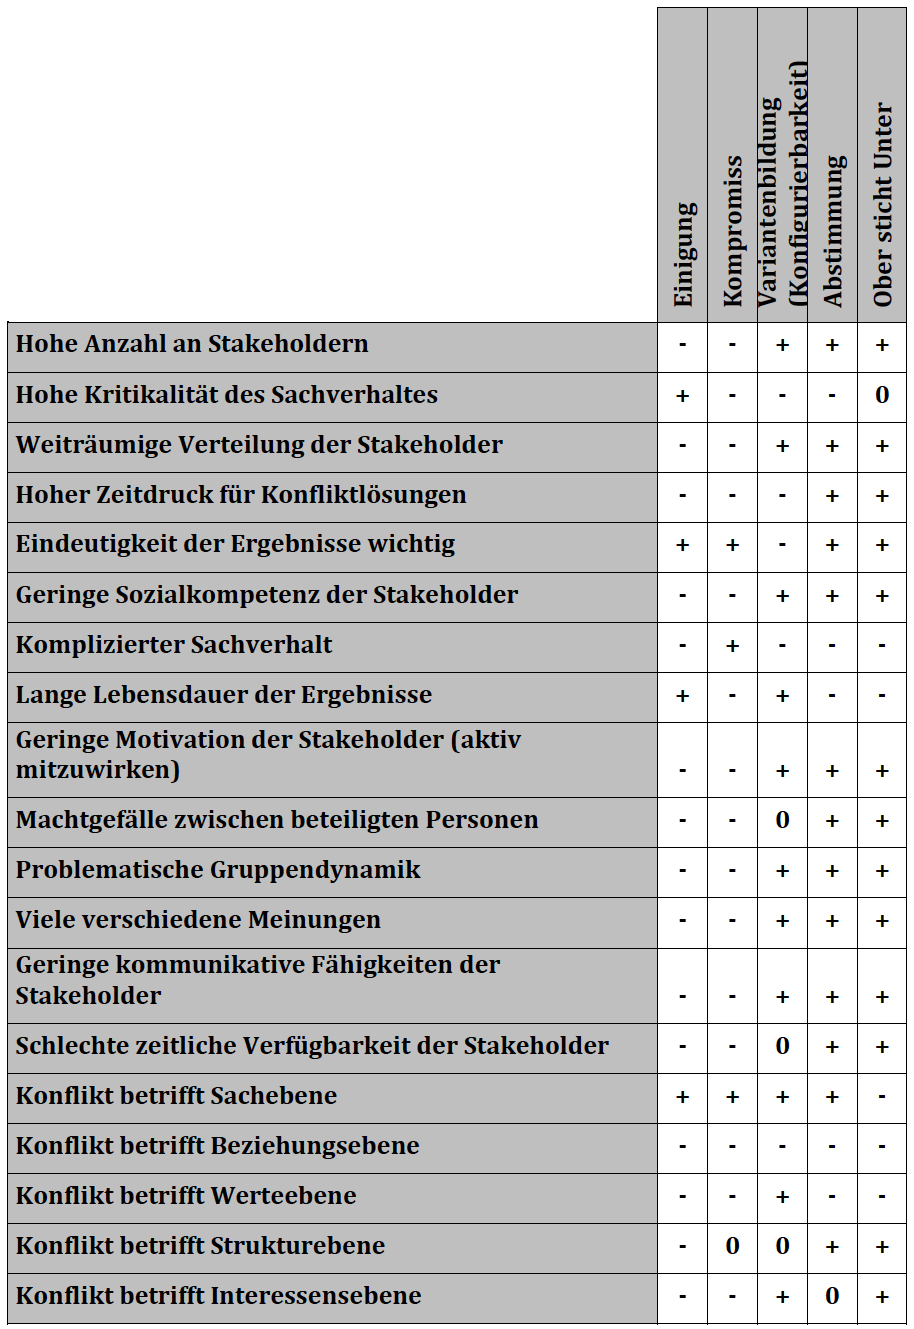
\includegraphics[width=0.8\textwidth]{images/KonsolidierungstechnikenTabelle}
    \caption{Konsolidierungstechniken}
    \label{fig:konsolidierungstechniken}
\end{figure}~\autocite[Abbildung 5][S.45]{OliverCreighton.2012}
  %! Author = philippkust
%! Date = 26.02.23

\subsection{Stakeholderanalyse}\label{sec:stakeholderanalyse-teil-1}
\subsubsection{Identifizierung von Stakeholdern}
Um eine Analyse der Stakeholder durchführen zu können, müssen diese Stakeholder zuerst identifiziert werden.
Ein Stakeholder kann dabei dadurch beschrieben werden, dass er ``eine Person oder eine Organisation [ist], die (direkt oder indirekt) Einfluss auf die Anforderungen des betrachteten Systems hat''\autocite[Seite 8]{Maulhardt.a}.
Um diese Personen und Organisationen zu identifizieren, gibt es verschiedene Methoden.

Zuerst sollte Brainstorming genutzt werden, um möglichst viele Stakeholder zu identifizieren.
Dazu wird insbesondere mit Personen geredet, welche direkt mit dem Projekt zu tun haben beziehungsweise damit zu tun haben werden.
Als Ergebnis entsteht eine erste Liste mit möglichen Stakeholdern, welche allerdings noch nicht dem Anspruch der Vollständigkeit gerecht werden kann.

Um die Liste der Stakeholder zu vervollständigen, kann nun mit der Analyse von vorhandenen Dokumenten begonnen werden.
Dabei werden alle Dokumente, welche mit dem Projekt zu tun haben, durchsucht und nach Stakeholdern ermittelt.
Insbesondere Verträge, die mit dem Projekt zu tun haben, bieten dabei einen guten Anhaltspunkt, da hier bereits Stakeholder genannt werden können.

Zuletzt ist eine Analyse der Produktentwicklung zu empfehlen.
Dabei können verschiedene Aspekte des Prozesses betrachtet werden, um Stakeholder zu identifizieren, indem man sich die folgenden Fragen stellt:

\begin{itemize}
    \item \textbf{Entwicklungsschritte:} Wer ist an den einzelnen Schritten der Entwicklung beteiligt?
    \item \textbf{Ressourcen:} Welche Ressourcen werden benötigt und wer stellt diese bereit?
    \item \textbf{Abhängigkeiten:} Welche Abhängigkeiten hat das Projekt von anderen Projekten beziehungsweise von anderen Personengruppen?
    \item \textbf{Ergebnisse:} Wer ist an den Ergebnissen des Projekts interessiert?
\end{itemize}

Die Stakeholder unterscheiden sich natürlich stark bei unterschiedlichen Projekten.
Allerdings kann gesagt werden, dass die Benutzer des Produkts sowie die Erwerber quasi ein minimales Set an Stakeholdern darstellen.
Zwei weitere Gruppen stellt zum einen die Organisation, welche das Produkt entwickelt und zum anderen regulatorische Behörden dar\autocite[vgl.][Seite 8]{ISONorm.a}.

\subsubsection{Analyse der Stakeholder}
Nachdem die Stakeholder identifiziert wurden, können diese nun analysiert werden.
Dabei werden die Stakeholder nach verschiedenen Kriterien eingeteilt, um die Bedeutung der Stakeholder für das Projekt zu ermitteln.

Eine übliche Methode ist die Einordnung der Stakeholder in die Power-Interest Matrix, welche von Aubrey Mendelow entwickelt wurde.
Diese Matrix stellt die Stakeholder in Abhängigkeit von ihrer Macht und ihrem Interesse an dem Projekt dar\autocite[vgl.][Seite 6f]{Botten.2006}.

\begin{figure}[ht]
    \centering
    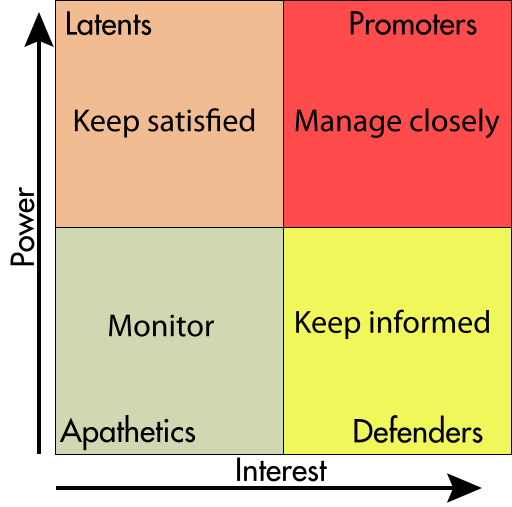
\includegraphics[width=0.3\textwidth]{Stakeholders_matrix}
    \caption{Power-Interest Matrix von Aubrey Mendelow}
    \label{fig:power-interest-matrix1}
\end{figure}

Mit diesen vier verschiedenen Gruppen muss jeweils unterschiedlich umgegangen werden.

\begin{itemize}
    \item \textbf{Apathetics:} Durch den geringen Einfluss und die geringe Macht ist diese Gruppe leicht zu überzeugen, weshalb sie eine eher geringe Beachtung finden.
    \item \textbf{Defenders:} Diese Gruppe ist zwar nicht besonders stark, hat aber ein starkes Interesse an dem Projekt.
        Da diese Gruppe es auch schaffen kann, Gruppen mit mehr Einfluss zu überzeugen, sollten diese Stakeholder in die Prozesse eingeschlossen werden und dadurch davon überzeugt werden, dass das Projekt für sie von Vorteil ist.
    \item \textbf{Latents:} Da diese Gruppe zwar viel Einfluss hat, aber kein Interesse an dem Projekt hat, sollte verhindert werden, dass diese Gruppe zu Promotern wird.
        Dies kann durch eine gute Kommunikation erreicht werden, um die Vorteile des Projekts zu verdeutlichen.
    \item \textbf{Promoters:} Bei dieser Gruppe muss unterschieden werden, ob diese dem Projekt positiv oder negativ gegenübersteht.
        In beiden Fällen ist es allerdings notwendig, durch ausreichend Lehre/Kommunikation diese Gruppe zu überzeugen, dass das Projekt notwendig ist.
        Anschließend sollte auch mit dieser Gruppe diskutiert werden, wie man das Projekt am besten umsetzt, um auch deren Eindrücke in das Projekt einfließen zu lassen.
\end{itemize}

Eine weitere Methode zur Einordnung der verschiedenen Stakeholder ist das Hervorhebungs-Modell von Ronald Mitchell, Bradley Agle und Donna Wood.
Dieses Modell unterscheidet zwischen acht verschiedenen Arten von Stakeholdern, welche unterschiedliche Bedeutung für das Projekt haben.
Diese Unterscheidung wird durch eine Einordnung in Kategorien Power, Legitimität und Dringlichkeit vorgenommen.
Dabei wird analysiert, wie viele von den genannten Kategorien auf die einzelnen Stakeholder zutreffen.

\begin{figure}[ht]
    \centering
    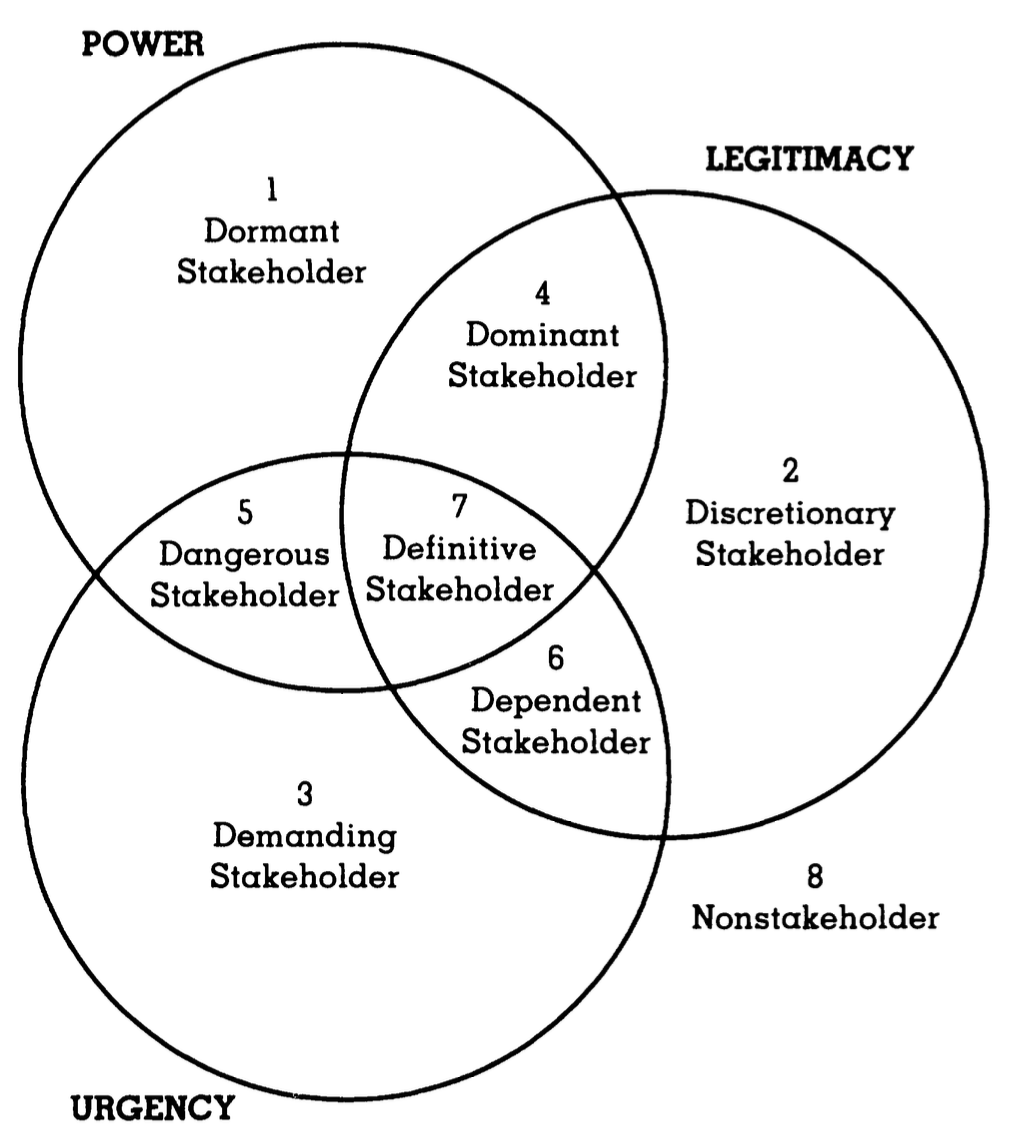
\includegraphics[width=0.3\textwidth]{Salience-Model}
    \caption{Hervorhebungs-Modell von Ronald Mitchell, Bradley Agle und Donna Wood\autocite[Seite 874]{Mitchell.1997}}
    \label{fig:highlight-model}
\end{figure}

Personengruppen, auf die eine von den drei Kategorien zutrifft, werden als latent eingestuft.
Diese müssen aufgrund ihrer begrenzten Zeit, Energie und anderer Ressourcen vom Management nicht unbedingt berücksichtigt werden.

Personengruppen, auf die zwei von den drei Kategorien zutreffen, werden als potenziell wichtig eingestuft.
Diese sogenannten ``erwartenden'' Stakeholder sind aktiv und haben ein Interesse an dem Projekt.
Dementsprechend sollte der Austausch zwischen den Projektleitern und diesen Stakeholdern intensiviert werden.

Die wichtigsten Stakeholder sind diejenigen, auf die alle drei Kategorien zutreffen.
Dabei ist auch darauf zu achten, ob erwartende Stakeholder zu dieser Gruppe aufsteigen, da nur ein Attribut fehlt, um dieser Gruppe zugeordnet zu werden.
Mit diesen sollte ein intensiver Austausch gepflegt werden und auf Anmerkungen dieser Gruppe mit entsprechender Priorität reagiert werden\autocite[vgl.][Seite 874ff]{Mitchell.1997}.



  \section{Durchführung der Anforderungsanalyse}
\subsection{Stakeholderanalyse}
Nachdem bereits geklärt wurde, wie eine Stakeholderanalyse durchgeführt werden kann, soll diese nun auch für das Projekt beschrieben werden.
Das Brainstorming hat ergeben, dass in erster Linie die \textbf{Benutzer} des Produkts sowie die \textbf{Erwerber} als Stakeholder in Betracht gezogen werden müssen.
Die Benutzer sind dabei vornehmlich männlich\autocite[vgl.]{Ailon.a} und in der Altersgruppe von 18 bis 40 Jahren anzusiedeln\autocite[vgl.]{Ailon.b}.
Zudem ist die \textbf{Organisation}, welche das Produkt entwickelt, sowie regulatorische Behörden ebenfalls als Stakeholder zu betrachten.

Darüber hinausgehende Stakeholder sind die \textbf{Rechteinhaber} der Filme, welche auf der Seite präsentiert werden sollen.
Da diese die Vorgaben machen, welche Sicherheitskriterien gegen Piraterie erfüllt werden müssen, sind diese ebenfalls als Stakeholder zu betrachten.

Die weiterführende Analyse der Dokumente hat ergeben, dass zusätzlich auch die \textbf{Investoren} in die Firma des Kunden Stakeholder sind.
Diese Geldgeber sind für die Finanzierung des Projekts verantwortlich und können dementsprechend Einfluss auf die Anforderungen nehmen.
Ebenso sind \textbf{regulatorische Behörden} zu berücksichtigen, da diese die Einhaltung der gesetzlichen Vorgaben überprüfen.

Die Analyse der Produktentwicklung hat zuletzt noch ergeben, dass auch die \textbf{Entwickler} des Produkts als Stakeholder betrachtet werden müssen.
So sind diese dafür verantwortlich, dass das Produkt den Anforderungen entspricht und die Anforderungen in der Dokumentation korrekt beschrieben sind.

Somit ergeben sich folgende Stakeholder:
\begin{itemize}
    \item Benutzer
    \item Kunde/Erwerber
    \item entwickelnde Organisation
    \item Regulatorische Behörden
    \item Rechteinhaber
    \item Investoren
    \item Entwickler
\end{itemize}

Diese Personengruppen sollen nun anschließend in einer Stakeholderanalyse betrachtet werden.
Zuerst ist die Einordnung in die Power-Interest Matrix vorzunehmen.
\begin{figure}[ht]
    \centering
    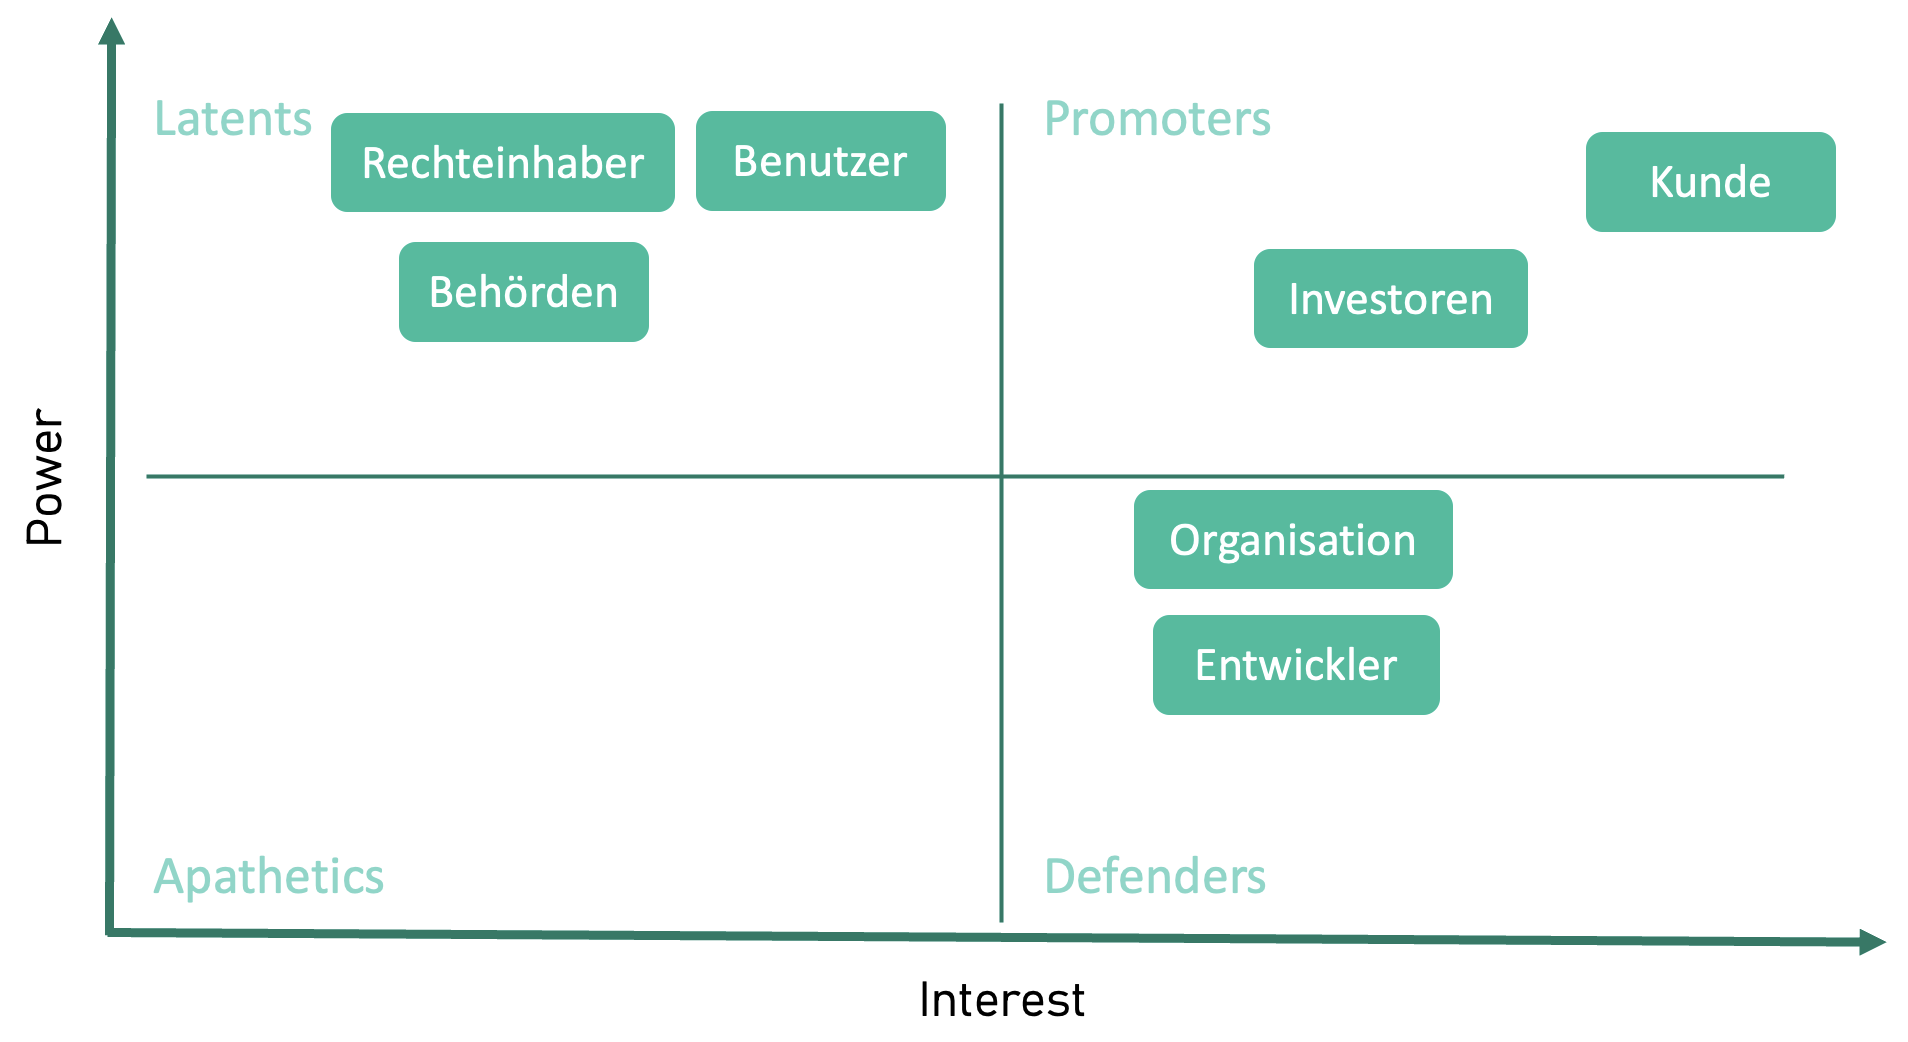
\includegraphics[width=0.7\textwidth]{Power-Interst-Matrix-Teil2}
    \caption{Power-Interest Matrix für die Stakeholderanalyse}
    \label{fig:power-interest-matrix2}
\end{figure}

Aus dieser geht hervor, dass die Kunden und die Investoren am meisten Macht sowie Interesse an dem Projekt haben.
Somit sollten diese sehr eng in das Projekt eingebunden werden und die Einwicklung des Produkts mitbestimmen.
Eine hohe Macht, ohne dabei ein besonders hohes Interesse zu haben, haben die regulatorischen Behörden, die Nutzer sowie die Rechteinhaber der Filme.
Alle drei Gruppen sind nicht direkt vom Ausgang der Entwicklung abhängig.
Die Benutzer beispielsweise haben auch Alternativen zum angebotenen Produkt, auch wenn dieses im optimalen Fall einen gewissen Mehrwert bieten soll.
Zuletzt sind die Entwickler sowie die Organisation, welche das Produkt entwickelt, in die Gruppe der Verteidiger einzuordnen.
Diese haben zwar ein hohes Interesse an dem Projekt, da Sie finanziell davon abhängig sind, jedoch bestimmt der Kunde über die Anforderungen an das Projekt.

Die Einordnung in das Hervorhebungsmodell kann bis zu einem gewissen Grad aus der Power-Interest Matrix abgeleitet werden.
So treffen auf die Benutzer sowie die Kunden alle drei Merkmale zu, weswegen sie als definitive Stakeholder eingestuft werden müssen.
Auf die Investoren treffen die Merkmale Macht und Legitimität zu, weswegen sie als erwartend eingeordnet werden können.
Die restlichen Stakeholder haben jeweils nur eins der drei möglichen Merkmale, wodurch diese als latente Stakeholder gesehen werden können.
Die genaue Einordnung dieser restlichen Stakeholder ist in der folgenden Auflistung dargestellt:

\begin{itemize}
    \item entwickelnde Organisation: Legitimität
    \item Regulatorische Behörden: Macht
    \item Rechteinhaber: Macht
    \item Entwickler: Legitimität
\end{itemize}

Nun müssen die Stakeholder nach Ihren Anforderungen an das Produkt eingeteilt werden.
So ist für die Benutzer ein einfaches und intuitives Interface wichtig, sodass diese die Filme möglichst einfach finden und wiedergeben können.
Die Kunden sowie die Investoren hingegen sind an einem möglichst hohen Umsatz interessiert.
Deswegen ist es ihnen wichtig, dass zum einen die Kunden möglichst zufrieden sind, allerdings auch, dass die Entwicklungskosten möglichst gering sind.
Dies widerspricht sich allerdings mit dem Verständnis der entwickelnden Organisation und den Entwicklern, die eine hohe Qualität des Produkts anstreben.
Die regulatorischen Behörden sind an der Einhaltung der gesetzlichen Vorgaben interessiert, weshalb diese die Einhaltung der Sicherheitskriterien überprüfen wollen.
Zuletzt sind die Rechteinhaber an der Einhaltung der Sicherheitskriterien interessiert, da diese verhindern wollen, dass Kopien der Filme im Internet verbreitet werden.


  %%%%%%%%%%%%%%%%%%%%%%% Literaturverzeichnis %%%%%%%%%%%%%%%%%%%%%%%
  \phantomsection
\addcontentsline{toc}{section}{Literatur}
\printbibliography
\newpage


  %%%%%%%%%%%%%%%%%%%%%%%%%%%%%% Anhang %%%%%%%%%%%%%%%%%%%%%%%%%%%%%%
  \renewcommand{\thetable}{\Alph{section}.\arabic{table}}
  \renewcommand{\thefigure}{\Alph{section}.\arabic{figure}}
  \renewcommand{\thelstlisting}{\Alph{section}.\arabic{lstlisting}}
  \pagenumbering{Alph}

  \begin{appendix}
  \section{Anhang}
\end{appendix}
\end{document}